\section{Introducere}

Scopul acestui proiect este acela de a implementa alți algoritmi de căutare pentru a-l ajuta pe Mr. Pacman să găsească mâncarea în cel mai scurt timp. Vom face și o comparație între cei 2 algoritmi noi (Un algoritm bidirecțional și Weighted A*) și cei 4 deja reprezentați în laboratoarele anterioare ( BFS, DFS, A* și UCS) . \newline


\subsection{Definirea problemei și soluționarea acesteia}

Prin compararea mai multor algoritmi de căutare vrem să rezolvăm problema găsirii drumului spre mâncare în cel mai scurt timp. 
\newline
\newline
Adițional am mai creat-o și pe Miss Pacman, jucându-ne cu grafica Pacmanului original, adăugând o fundiță, gene și ochi albaștrii ce se deplasează odată cu Miss Pacman. 

\subsection{Algoritmii folosiți}

\begin{enumerate}
  \item Bidirectional Algorithm
  \item Weighted A* 
  \item BFS, DFS, UCS, A*
\end{enumerate}
\newline
Algoritmii de căutare DFS, BFS, UCS și cel bidirecțional sunt algoritmi neinformați(constă în explorarea alternativelor, fără a utiliza informații specifice despre problemă).
\newline
\newline
Algoritmii de căutare A* și Weighted A* sunt algoritmi informați(euristică-încearcă alegerea „inteligentă” a nodurilor care trebuie expandate).
\newline

\begin{figure}[h]
    \centering
    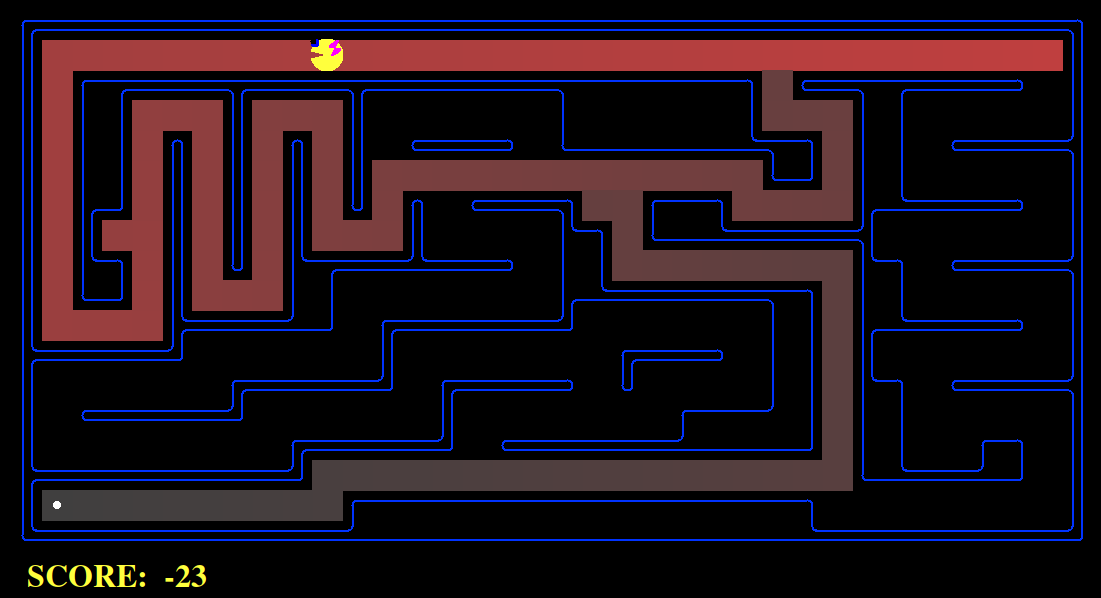
\includegraphics[width=16cm]{text/images/pic1.png}\\
    \caption{Medium Maze Miss Pacman}
\end{figure}



